%--------------
\section{Research questions}
This thesis addresses conceptual issues at the intersection of tide prediction and mesoscale oceanography, with practical implications for operational sea level forecasting practice. 
In contrast to the canonical numerical approach to coastal sea level that broadly pursues  ever-higher resolution simulations, this work turns to focus on the less-studied but relevant value offered by established operational systems; especially at the ocean mesoscale. Addressing the representation of sea level at the intersection of existing systems is important for building the foundations of future multi-model seamless forecasting services.


\emph{%
Is the operationalisation of high resolution coastal simulations a prerequisite for providing regular sea level forecasts?  Despite comparatively low coastal resolution, can \BL{} directly provide useful prognosis of non-tidal coastal sea level and with what limitations? }



\emph{Are point-by-point tide-gauge observations the only relevant basis on which to compare and assess heterogeneous sea level forecast simulations? 
Why is the role of coastally trapped waves prominent in the oceanographic literature but seemingly absent from operational forecasting?}



\emph{Has numerical simulation rendered conventional tide prediction redundant for operations?  How can the unique traditional function of tide prediction compliment nominally non-tidal ocean forecasts and future seamless prediction systems? 
}


%--------------------------------------------------
\section{Observable sea level and forecasts}

Sea level plays a unique role in physical oceanography and forecasting thanks at least in part to its very \emph{observability} \citep{Wilson:2010hy}. 
Variations in coastal \emph{still water level} \citep{Pugh:2014di} reflect a diverse range of hydrodynamic phenomena operating across time and length scales.   Furthermore the relative significance of the pheneomena vary greatly in space and time.
\citet{10.1007/s10712-019-09531-1} recently reviewed this diverse mix of physical phenomena present in the observations and note that ``\textit{it is mistake to think that coastal sea level variability always has a ‘local’ forcing (although it often does).}''. 
Figure \ref{fig:sealevelScales} provides a schematic summary of the physical time and length scales of broad classes of these phenomena that contribute to ocean water level variations, taking inspiration from similar diagrams in \citet{10.1007/s10712-019-09531-1} and \citet{Chelton:2001ws}.
%-----------------------------
\begin{figure}[H]\centering
  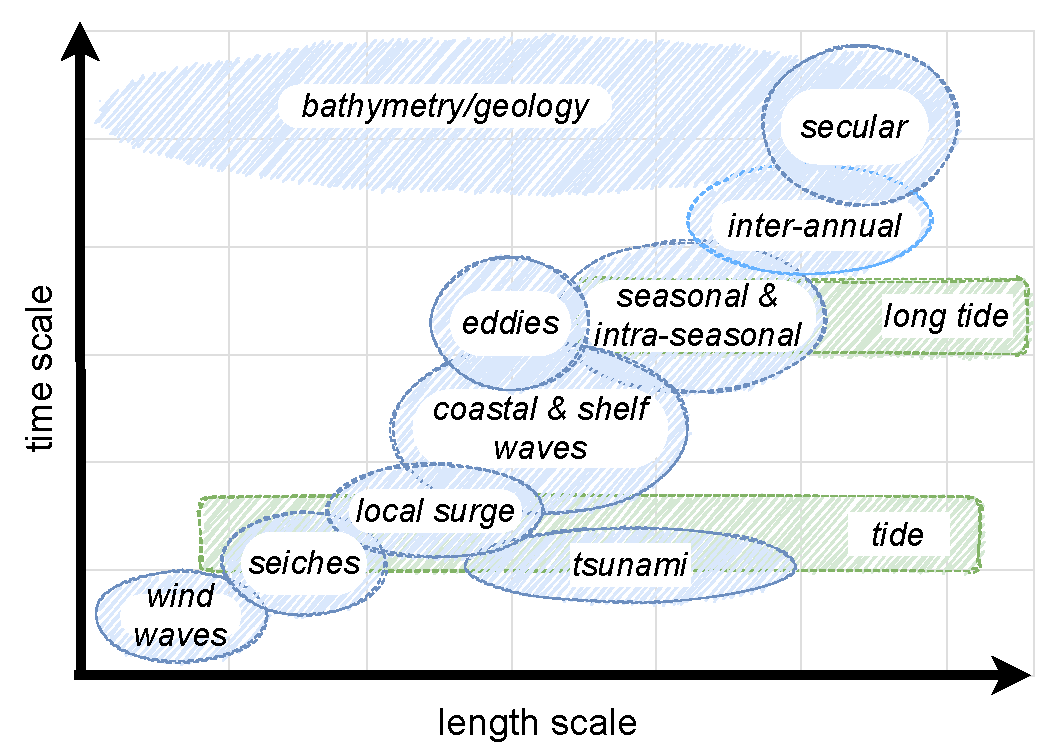
\includegraphics[width=\figwidthFull]{figures/diagrams/scales_time_length.pdf}
  \caption{Schematic indication of the relative time and length scales of a range of physical processes contributing to observable coastal sea level.}
  \label{fig:sealevelScales}
\end{figure}
%-----------------------------
The visual differentiation of tides from the other phenomena in Figure \ref{fig:sealevelScales} is intentional.  Tides have unique properties; but exactly what is designated as tidal in an operational context can be more ambiguous than first impressions imply. This topic is unpacked further in section \ref{sec:tide_intro}. Tides in the schematic are seen to span from very short to very long length-scales but at more restricted frequencies than other phenomena.    Furthermore, the long period tides are are shown separately in anticipation of a later discussion of how these species are potentially problematic in some forecasting applications.

How the varying balance of phenomena is expressed in observed sea level is illustrated by the spectra shown in Figure \ref{fig:obsSpectraEg} for two Australian locations.   Variability at nominally tidal frequencies is a striking feature at nearly all coastal locations;  ``the [tidal] constituent lines emerge from the noise background as trees from the grass'' \cite{godin:1972}.
Observed power at tidal frequencies does not however provide a direct attribution to tidal forcing and the extent to which this matters for forecasting applications is a conceptual theme addressed in chapter \ref{chp:tideFlavours}.
%-----------------------------
\begin{figure}[H]\centering
	\subfloat[Darwin in Northern Australia - large diurnal tide.]{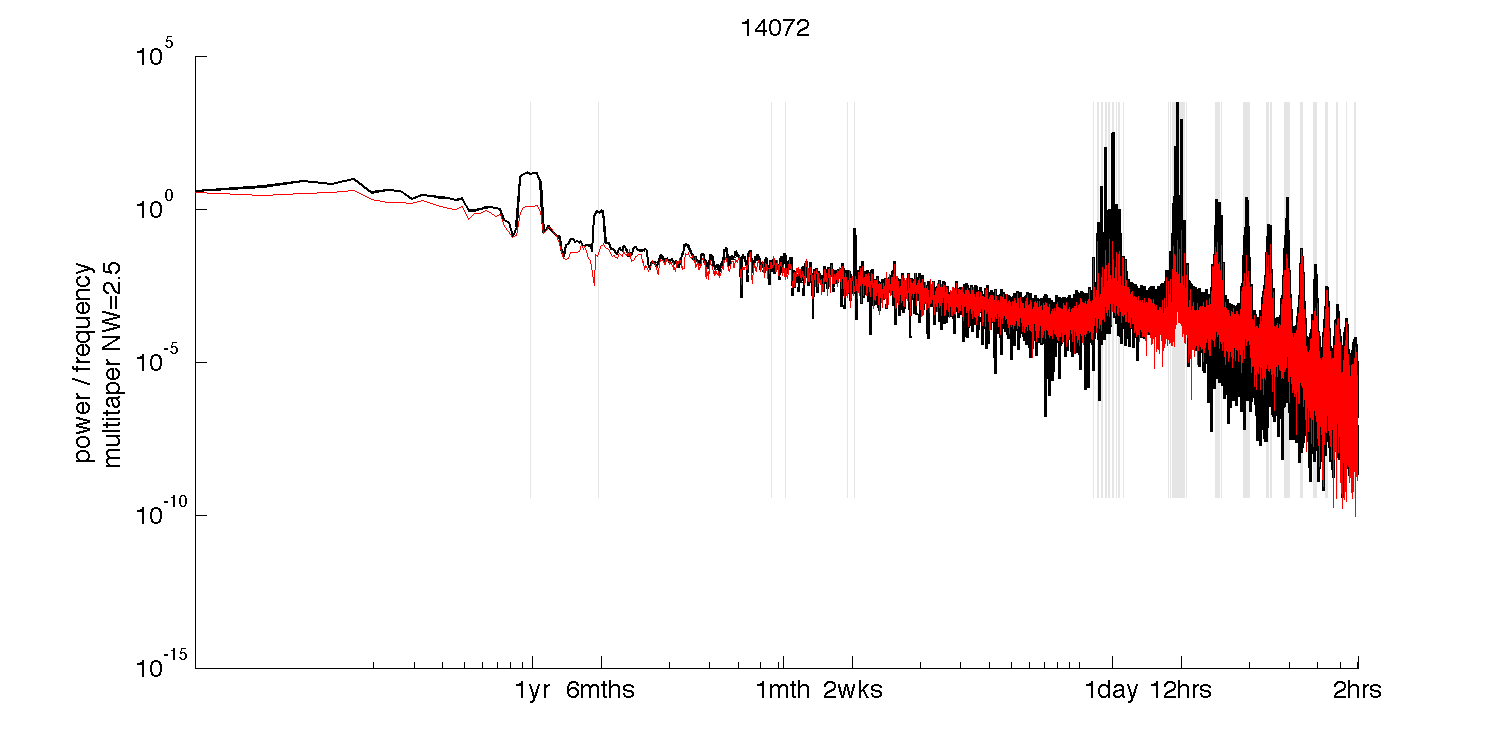
\includegraphics[width=\figwidthFull]{figures/plots/plot_14072.png}} \\
	\subfloat[Esperence in Southern Australia - powerful synoptic signal.]{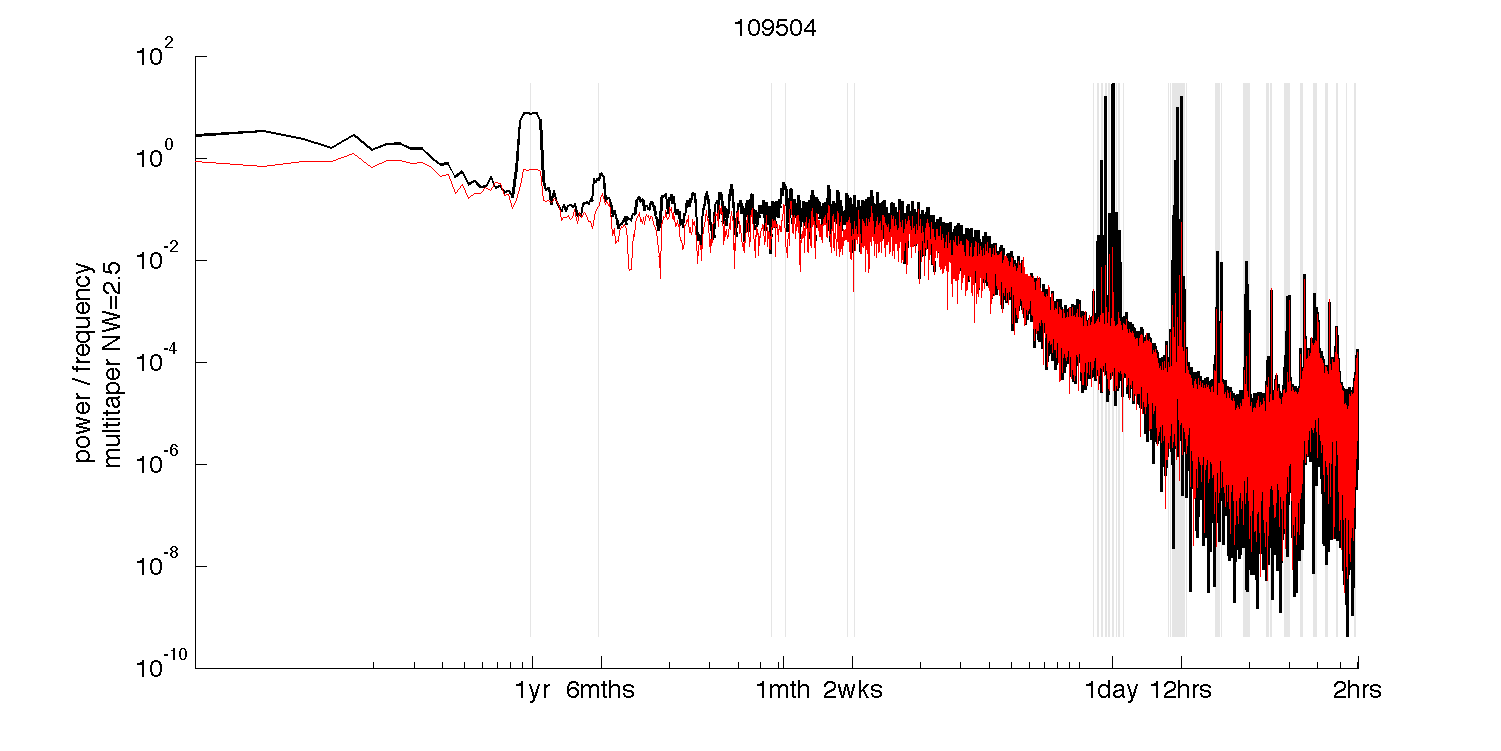
\includegraphics[width=\figwidthFull]{figures/plots/plot_109504.png}}
	\caption{Spectral estimates from two coastal tide gauges. Hourly data, black = observations, red = tidal residual, nominally tidal frequencies are shown with shading. An example of a `mixed spectra' \citep{Percival:1998tw}, in the sense of that prominent tidal spectral lines appear to be embedded in a background continuum of coloured variability.}
    \label{fig:obsSpectraEg}
\end{figure}
%-----------------------------

Quantified observations of sea level currently available for operational use fall into essentially two categories: (1) insitu and (2) remote.    Figure \ref{fig:sealevelObsCartoon} illustrates this difference schematically.

Insitu observations from coastal tide gauges are by far the most established and studied source.    The availability of tide gauge observations is intrinsically connected to the history of sea level study and the development of forecasting techniques; the longer view of which is covered in the history of \citeauthor{Cartwright:2000tt}.
Typical tide gauge instruments in fact measure the `air gap' between a sensor and the water surface from which a relative level is derived \citep{PCTMSL-sp9}. 
But the very nature of why and how tide gauges are installed raises a list of special characteristics relevant to operational forecasting. These characteristics are variously considered to add complication or insight from the perspective of academic  differec
Coastal locations are subject to both global and spatially localised hydrodynamic effects; in addition to influences like sediment movement, riverine phenomena and even coastal engineering works.   
The limited extent to which the range of scales present in the tide gauge observations can be adequately represented by any forecast system is a fundamental characterisation discussed across chapters \ref{chp:aggregate},\ref{chp:waveguide}and \ref{chp:tideFlavours}.    
Tide gauge observations can be mapped to certain sea level impacts and decisions, though not always directly; as for instance in \cite{Hague:2019ha}. 
Commonly these observations are the basis of vertical reference information and geodetic derivations that are ultimately connected to the interpretation of any quantitative sea level forecast \citep{Woppelmann:2006un}\citep{AVWS2021}.
More comprehensive observations of sea level than are possible from tide gauges is listed as a key requirement for future development by \citeauthor{10.3389/fmars.2019.00437} and video-based systems in particular show promise \citep{10.1175/jtech-d-18-0203.1} and \cite{2018agufmep52d..26h}. 
%-----------------------------
\begin{figure}[H]\centering
  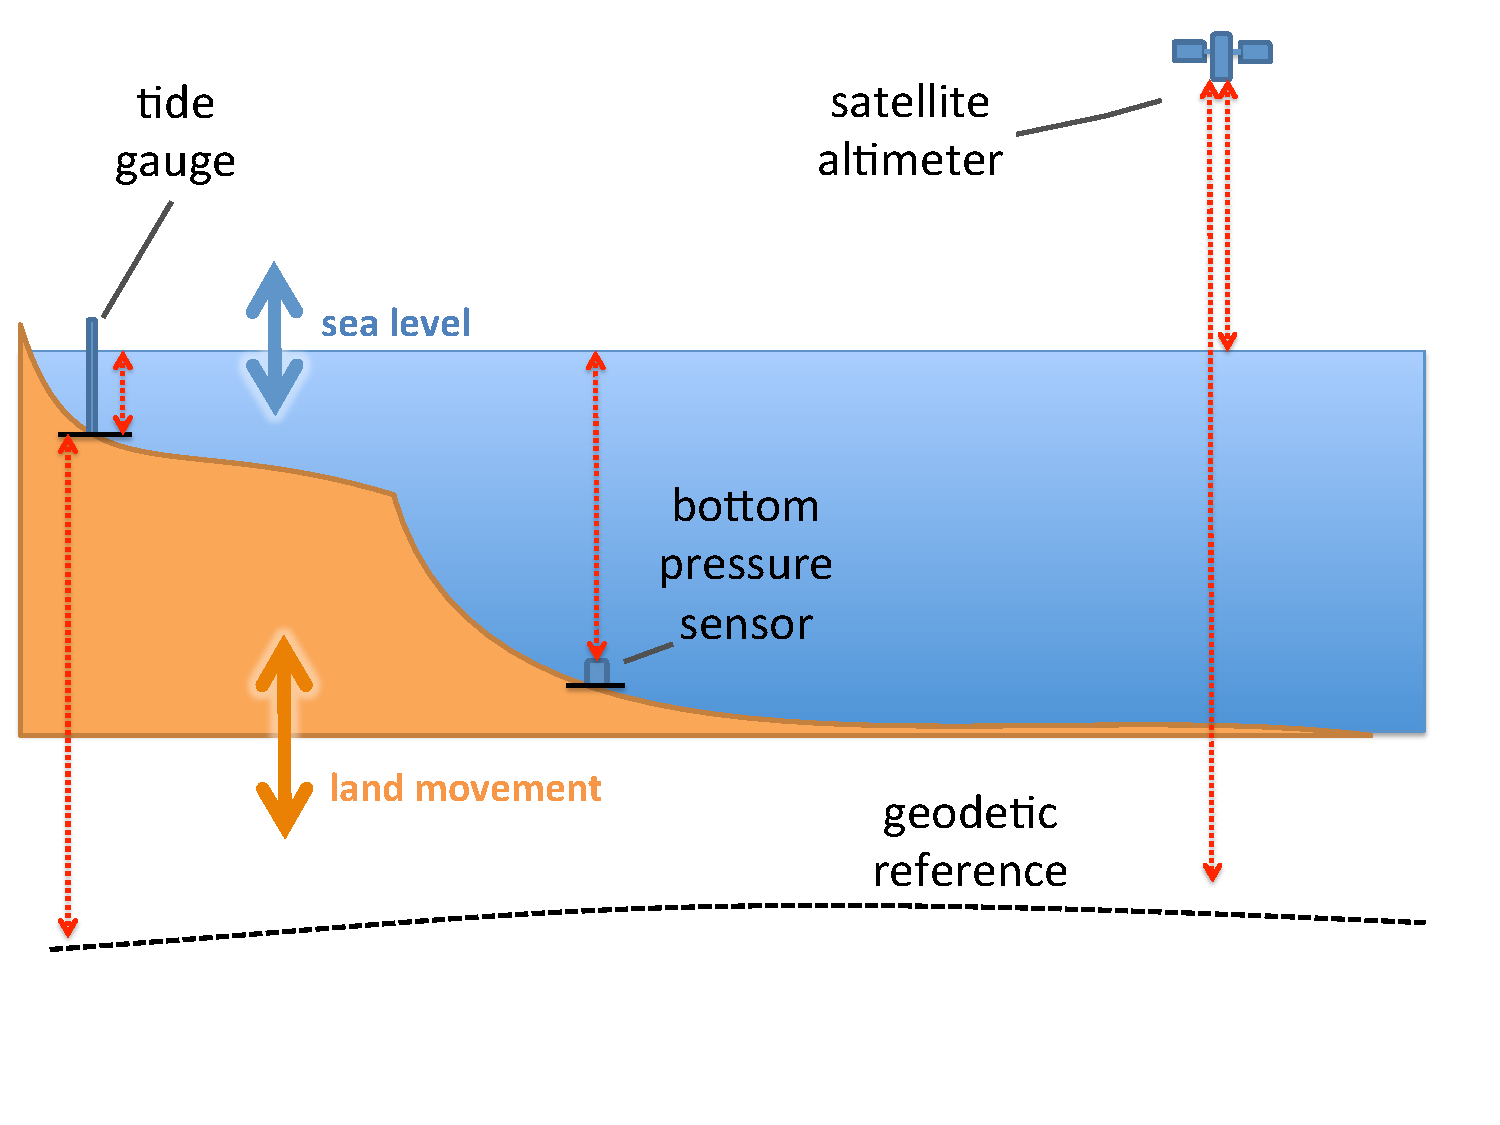
\includegraphics[width=\figwidthBig]{figures/diagrams/sealevel_cartoon.pdf}
  \caption{Simplified illustration of the relative nature of sea level and existing observing platforms.}
  \label{fig:sealevelObsCartoon}
\end{figure}
%-----------------------------
Remote observations of sea level are also derived from what is effectively a very large air-gap .   The derivation from active radar return signals to a meaningful sea level value is non-trivial but very mature away from the coast \citep{Fu:2001ub}.  Operational mesoscale oceanography is heavily dependant on altimeter observations across the global ocean and is discussed further in section \ref{sec:operational_oceanography}.  
Operational application of remote sea level observations near the coast is complicated by both the very presence of land within the sensing `footprint' as well as more powerful but shorter time and length scales of sea level variability \citep{Vignudelli:2011wl}.   Whilst this is a  rapidly advancing field, coastal altimetry effectively remains pre-operational and needs to solve the handling of fundamental details such as vertical reference datums \citep{10.3389/fmars.2020.549467}.
The active nadir radar architecture of satellite sea level observations of the last two decades is expected to undergo a qualitative change with the planned wide-swath altimeter missions starting with SWOT \footnote{\url{https://earth.esa.int/web/eoportal/satellite-missions/s/swot}, \url{https://auswot.org/}}.   Wide swath observations of sea level remote observations promise to radically impact water level forecasting in the longer term but can not hope to become operationally relevant for some years to come. 

Operationally-relevant observations of sea level suffer from additional limitations that can be handled differently in more academic settings.   The most basic limitations are whether observations are accessible in near-real-time and the extent to which appropriate metadata is available and up to date.  
Quality control of observations is challenging task that is applied differently between an operational setting as for important long term historical archive projects \footnote{such as \url{www.gloss-sealevel.org}, \url{uhslc.soest.hawaii.edu} and \url{www.gesla.org}}.

The de-facto network of tide gauges from which sea level observations are provided to the Bureau of Meteorology are operated by a range of port authorities, state agencies and the Bureau itself. Inhomogeneity of tide gauge data quality is expected to be a permanent feature of operations; a status that is argued to be a core value of traditional tide prediction services in chapter \ref{chp:tideFlavours}. All evaluations made against tide gauges in this thesis are intentionally based on the Bureau's own operational archive.

%--------------------------------------------------
\subsection{Unique perspective of the operational setting}
\label{S:operational_setting}

The Australian Bureau of Meteorology is an \emph{operational} forecasting agency with characteristics that fundamentally frame the present study. The operational setting involves:
\begin{itemize}
    \item a finite suite of foundational forecasting systems;
    \item a diverse range of downstream applications;
    \item reliance on real-time and imperfect observations;
    \item regular and continuous schedule of forecast production;
    \item a preference for reliability over fidelity;
    \item a slow development and system change cycle.
\end{itemize}
This setting provides a perspective on geophysical fluid simulations that thus differs from broader academia as well as more single-purpose commercial forecasting.   As a result it could be said that this thesis does not launch neatly from a single academic `conversation' \citep{Booth:2009vy} but rather will draw on both peer-reviewed literature as well as internal Bureau of Meteorology inputs where relevant.
Unfortunately operational documentation often falls far behind aspirations.  The practive..... TBC   ...Tidal observation manuals exist eg \citep{IOC:2005tj}, \citep{Level:2011wu}, \citep{Parker:2007wq}.  However, analysis methods and design justifications are less formally documented - if at all.  The IOC understates this situation simply: `many organizations have developed their own method of tidal analysis'\citep{IOC:2005tj}\\

\begin{figure}[H]\centering
  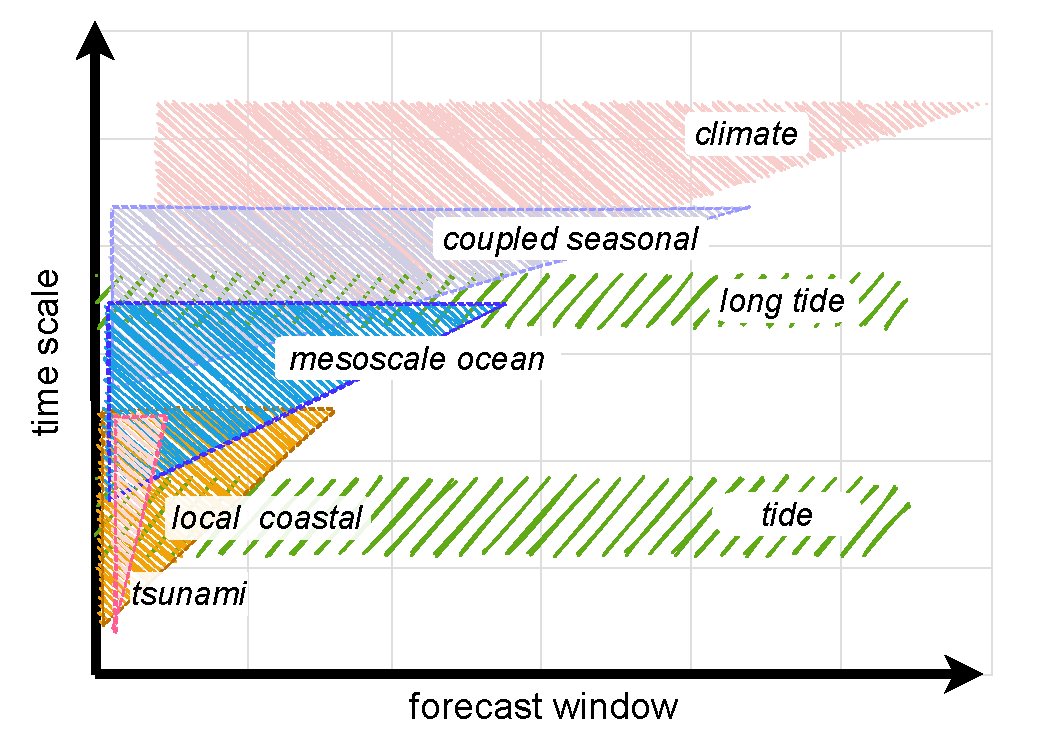
\includegraphics[width=\figwidthBig]{figures/diagrams/scales.pdf}
  \caption{Forecasting suite schematic with overlapping scales}
  \label{fig:SCALES}
\end{figure}



TBC - name why this raises PROBLEMS that are worth study ....

%--------------------------------------------------
\subsection{Relevance of restricted scope}

Compare to event based or behind real time studies ...


In contrast to the :
focus on extreme events
direction towards ever-higher resolution simluations.


Cite some on both global and Australian scale...


Viewing the
This thesis intentionally addressess the topic of routine forecasts of coastal sea level 
...
not to detract from the inevitable pursuit of ``comprehensive ...coastal '' 



\begin{figure}[H]\centering
  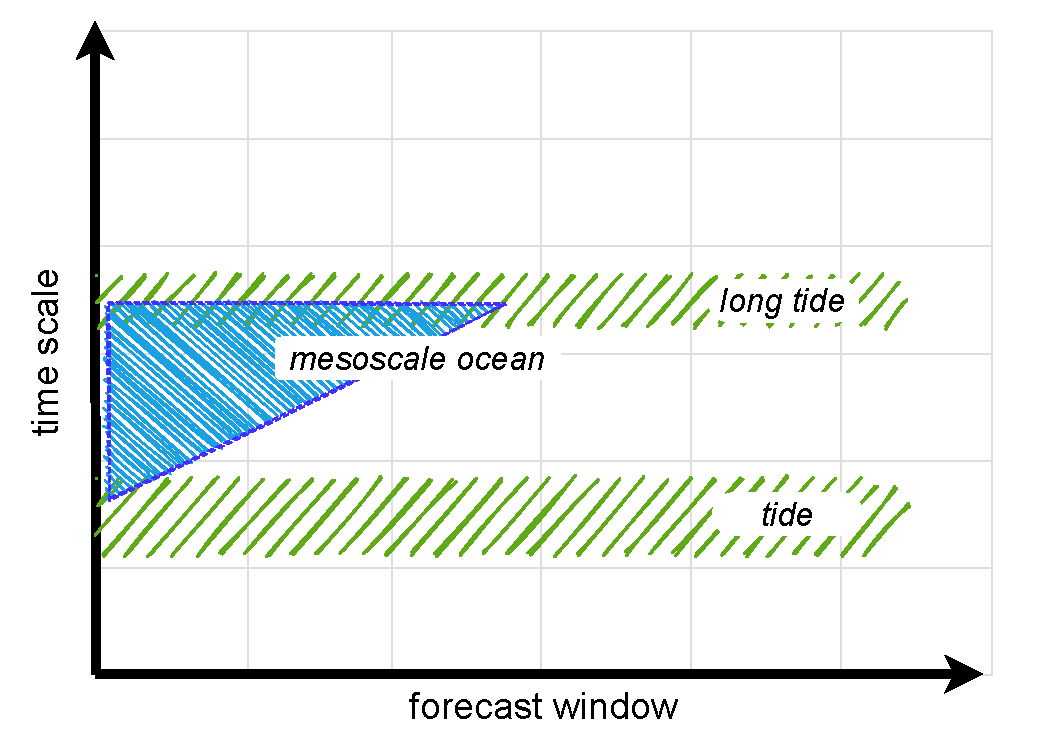
\includegraphics[width=\figwidthBig]{figures/diagrams/scales_focus.pdf}
  \caption{Focus on mesoscale and tidal scales overlap}
\end{figure}

set benchmarks and address some representation issues at the overlap of conventional tides and large scale ....

%--------------------------------------------------
\subsection{Preparing for seamless forecasts}

BoM research strategy.


More general:

\begin{itemize}
  \item Towards 'concrete' , increasingly realistic and inclusive primitive equation forward models.
Peterson M1 ]\citep{Petersen:2012tr}
 \item Towards data-driven, service target - idealised, simple and robust 
\end{itemize}




Tidal harmonic methods have for many decades provided the only routine source of sea level forecast - and with great success.  
In contrast, time stepping primitive equation dynamic models and data assimilation are relatively new arrivals to operational centres.  
These represent two qualitatively different perspectives on sea level prediction.\\


Over the past decade, the operational evolution of \OGCM-based prediction has increasingly brought the two approaches into something akin to Gallison's `trading zone' \citep{Galison:1996uc}.
Developments promise only to increase the amount of overlap into the previously independent practices of harmonic analysis, eg \cite{Arbic:2010us}.\\
Here Munk and Cartwright's aphorism from the 1960's regarding tidal analysis is illustrative:
\begin{quote}
  \dots predicting and learning are in a sense orthogonal, and the most interesting effects are those that cause the most trouble with a forecasting: the continuum, the nongravitational tides, and the non-linear interactions.\citep{Munk:1966ts} 
\end{quote}
Forecasts from \BL{} and other similar systems now represent sea level attributable to exactly these troublesome areas; or at least some physical subset therein.
Jayne's reference to the ``vexing problems'' \citep[pp812]{Jayne:2001tr} arising from applying frequency-domain theory in time-domain numerical tide modelling is illustrative.

\begin{figure}[H]\centering
  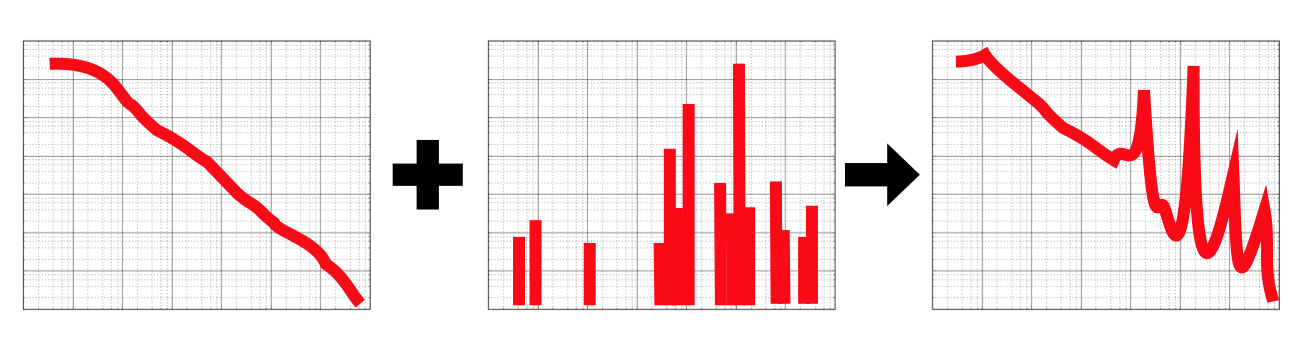
\includegraphics[width=\figwidthBig]{figures/diagrams/spectra_cartoon_1.png}
  \caption{Conventional decomposition concept: mixed sea level spectra comprising discrete tidal `lines' and red turbulent continuum.  Implementation of this concept has ramifications for sea level forecasting.}
  \label{fig:SPECTRA_CARTOON}
\end{figure}

Viewing sea level as a stationary set of harmonics is at face value quite at odds with a view of the ocean as a turbulent fluid.   In that sense, Gallison's portrayal of physics as `neither unified nor splintered into isolated fragments' \citep[pp 782]{Galison:1987wh} is apt.  Thus also is Peterson's assertion of `\dots{} the fundamental plurality of \dots{} scientific practice' \cite{Petersen:2012tr}. 
